\documentclass[8pt]{report}
\usepackage{amsmath, xfrac, enumitem, graphicx, ulem, float, bigints, bm, textcomp}
\usepackage{titlesec, mathtools}
\usepackage[margin=0.7in]{geometry}
\graphicspath{ {images/} }
\linespread{0.8}
\title{\Huge{\textsc{Strength of Materials - GATE}}}
\author{\huge{\textbf{Kulasekaran}}}
\begin{document}
\maketitle
\tableofcontents
%-----------------------------------------------------------------------------------------%
\chapter{Composition, Resolution and Equilibrium of Forces}
\section{Force}
	\begin{itemize}
		\item It is the action of one body on another that changes the state of being (rest/uniform motion) of the object on which it is being applied
		\item 3 things are needed to define a force: Magnitude, direction, Point of application
		\item According to Newton's first law: $\boxed{Force = Mass\;*\;Acceleration}$
	\end{itemize}\hrulefill
\section{Force systems}
	\begin{itemize}
		\item \textbf{Coplanar} - 2D system
		\item \textbf{Non-Coplanar} - 3D system
	\end{itemize}
	\subsection{Collinear}
		\begin{itemize}
			\item Two are more forces whose line of action is same
			\begin{figure}[H]
				\centering
				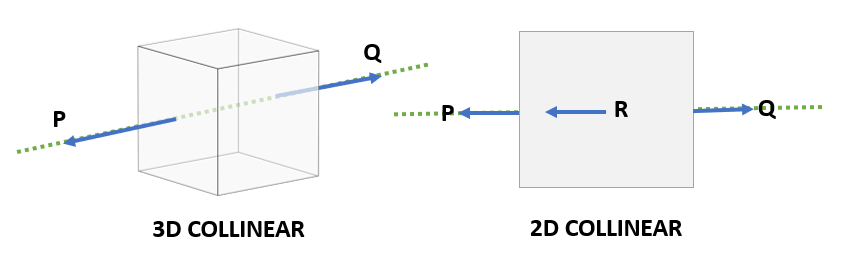
\includegraphics[scale=0.5]{collinear.png}
			\end{figure}
		\end{itemize}
	\subsection{Concurrent}
		\begin{itemize}
			\item Two are more forces which meet at a common point
			\begin{figure}[H]
				\centering
				\includegraphics[scale=0.2]{3dconcurrent.png}
				\includegraphics[scale=0.4]{2dconcurrent.png}
			\end{figure}
		\end{itemize}
	\subsection{Coplanar}
		\begin{itemize}
			\item Forces that are on the same plane
		\end{itemize}
	\subsection{Coplanar Concurrent}
		\begin{itemize}
			\item Forces that are on the same plane and meet at a common point as well
		\end{itemize}
	\subsection{Non-Coplanar Concurrent}
		\begin{itemize}
			\item Forces are not on the same plane but meet at a common point
		\end{itemize}
	\subsection{Coplanar Non-Concurrent}
		\begin{itemize}
			\item Forces are on the same plane but don't meet at a common point
		\end{itemize}
	\subsection{Non-Coplanar Non-Concurrent}			
		\begin{itemize}
			\item Forces are neither on the same plane nor meet at a common point
		\end{itemize}\hrulefill
%-----------------------------------------------------------------------------------------%
\section{Triangular Law of forces}
	\begin{itemize}
		\begin{figure}[H]
			\centering
			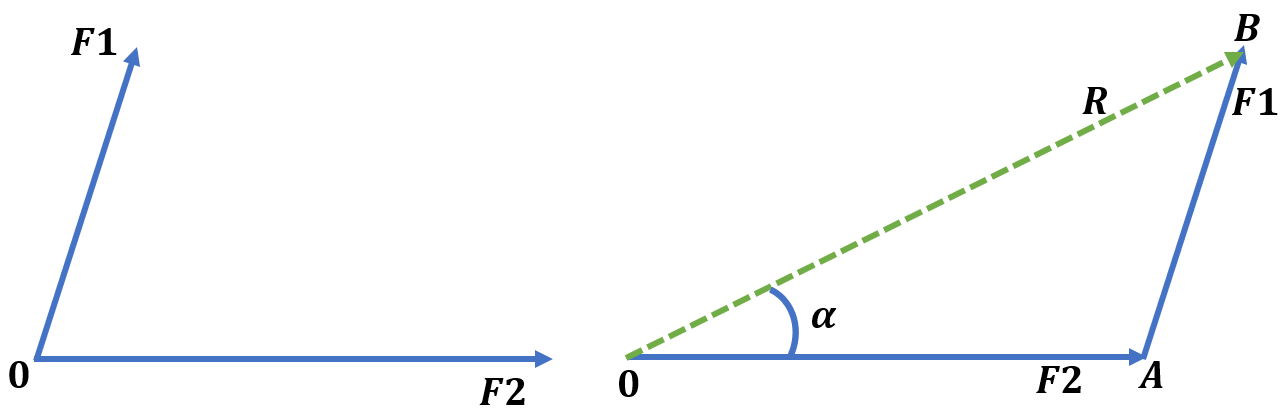
\includegraphics[scale=0.4]{triangularlaw.png}
		\end{figure}
		\item \textit{Two concurrent forces acting on a body is represented in magnitude and direction by two sides of a triangle taken in order, then their third side will represent the resultant of two forces in the direction and magnitude taken in opposite order}
		\item[] $$\boxed{R=\sqrt{F_1^2+F_2^2}}\;\;\boxed{\alpha=\cos^{-1}\left(\dfrac{F_1}{R}\right) = \sin^{-1}\left(\dfrac{F_2}{R}\right)}$$
	\end{itemize}\hrulefill		
%-----------------------------------------------------------------------------------------%
\section{Parallelogram Law of forces}
	\begin{itemize}
		\item \textit{If two concurrent forces are represented in magnitude as the two sides of a parallelogram, then the resultant of these two forces is the diagonal of the parallelogram}
		\begin{figure}[H]
			\centering
			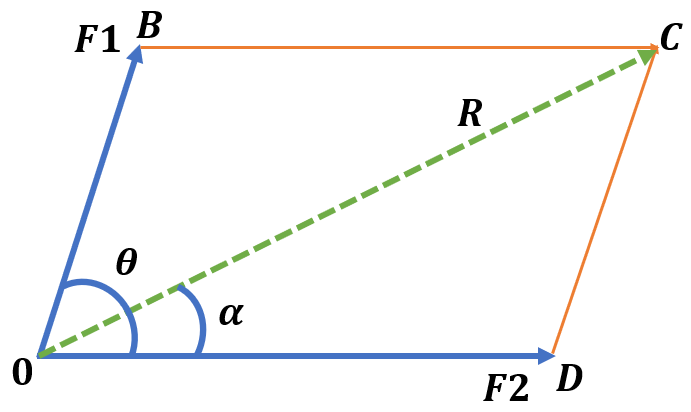
\includegraphics[scale=0.4]{parallelogramlaw.png}
		\end{figure}
		\item[] $$\boxed{R = \sqrt{F_1^2+2F_1F_2\cos\theta+F_2^2}}$$
	\end{itemize}\hrulefill
%-----------------------------------------------------------------------------------------%
\section{Polygon Law of forces}
	\begin{itemize}
		\begin{figure}[H]
			\centering
			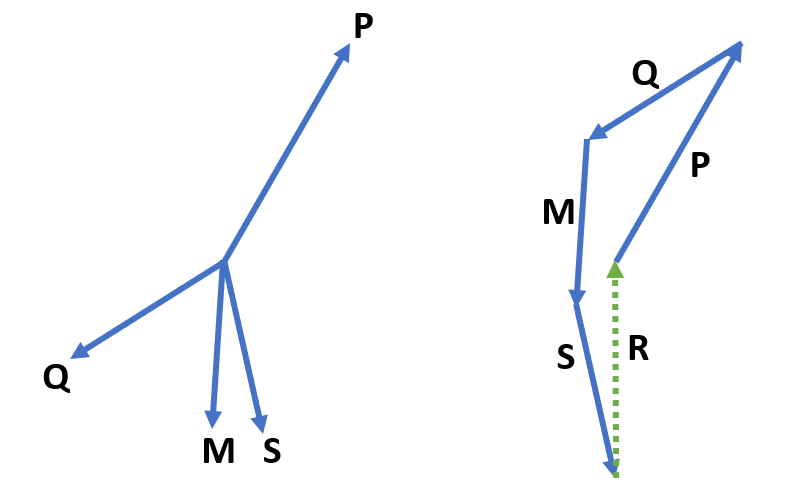
\includegraphics[scale=0.4]{polygonlaw.png}
		\end{figure}
		\item The triangular law can be extended to the polygon law. \textit{If a number of coplanar concurrent forces are represented in magnitude and direction by the sides of a polygon, taken in order, then their resultant can be represented by the closing side of the polygon}
	\end{itemize}\hrulefill
%-----------------------------------------------------------------------------------------%
\section{Resolution of Forces}
	\begin{itemize}
		\item The concept of replacing a single force at some angle with two of its component in the vertical and horizontal direction is called Resolution of forces.
		\begin{figure}[H]
			\centering
			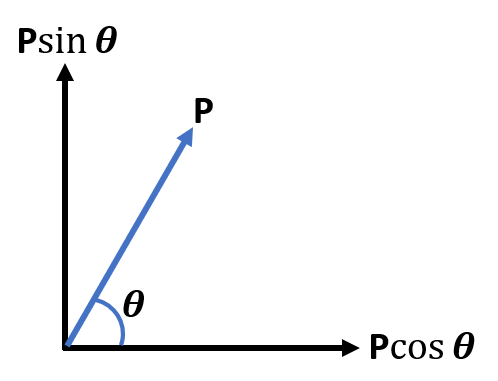
\includegraphics[scale=0.4]{resolution.png}
		\end{figure}
	\end{itemize}\hrulefill		
%-----------------------------------------------------------------------------------------%
\section{Equilibrium state}
	\begin{itemize}
		\item A body is said to be in equilibrium if it is at rest or moving with uniform velocity. \textbf{Under equilibrium state, the resultant of the force system will be zero.} 
	\end{itemize}\hrulefill
%-----------------------------------------------------------------------------------------%
\section{Lami's Theorem}
	\begin{table}[H]
		\begin{tabular}{cc}
			\parbox{4cm}{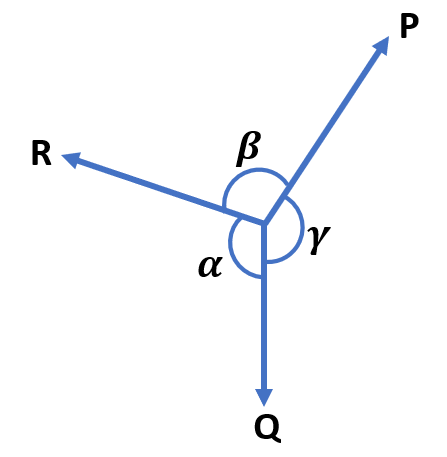
\includegraphics[scale=0.4]{lamistheorem}} &
			\parbox{12cm}{\textit{If 3 coplanar concurrent forces are in equilibrium, then each force is proportional to the sine of the angle between the other two sides}\\$$\boxed{\dfrac{P}{\sin\alpha}=\dfrac{Q}{\sin\beta}=\dfrac{R}{\sin\gamma}}$$}
		\end{tabular}			
	\end{table}\hrulefill
%-----------------------------------------------------------------------------------------%
\chapter{Analysis of Simple trusses}
	\begin{itemize}
		\item
	\end{itemize}
%-----------------------------------------------------------------------------------------%
\chapter{Friction}
	\begin{itemize}
		\item
	\end{itemize}
%-----------------------------------------------------------------------------------------%
\chapter{Work and Energy}
	\begin{itemize}
		\item
	\end{itemize}
%-----------------------------------------------------------------------------------------%
\chapter{Virtual work}
	\begin{itemize}
		\item
	\end{itemize}
%-----------------------------------------------------------------------------------------%
\chapter{Center of Gravity and Moment of Inertia}
	\begin{itemize}
		\item
	\end{itemize}
%-----------------------------------------------------------------------------------------%
\chapter{Impulse and Momentum}
	\begin{itemize}
		\item
	\end{itemize}
%-----------------------------------------------------------------------------------------%
\chapter{Lagrangian Equation}
	\begin{itemize}
		\item
	\end{itemize}
\end{document}
%-----------------------------------------------------------------------------------------%
%-----------------------------------------------------------------------------------------%
%-----------------------------------------------------------------------------------------%
